\documentclass[conference]{IEEEtran}
\usepackage[utf8]{inputenc}
\usepackage[spanish]{babel}
\usepackage{amsmath}
\usepackage{graphicx}
\usepackage{float}
\usepackage{circuitikz}
\graphicspath{{assets/}}
\IEEEoverridecommandlockouts
\raggedbottom
\def\BibTeX{{\rm B\kern-.05em{\sc i\kern-.025em b}\kern-.08em
    T\kern-.1667em\lower.7ex\hbox{E}\kern-.125emX}}

\begin{document}

\title{Taller de Física - Momento 2}

\author{
    \IEEEauthorblockN{1\textsuperscript{st} Kevin Ramírez Corrales}
    \IEEEauthorblockA{\textit{Universidad Cooperativa de Colombia}\\
    kevin.ramirezcorr@campusucc.edu.co}
    \and
    \IEEEauthorblockN{2\textsuperscript{nd} Mauro Jaramillo Zapata}
    \IEEEauthorblockA{\textit{Universidad Cooperativa de Colombia}\\
    mauro.jaramillo@campusucc.edu.co}
    \and
    \IEEEauthorblockN{3\textsuperscript{rd} Sofía Valero Loaiza}
    \IEEEauthorblockA{\textit{Universidad Cooperativa de Colombia}\\
    sofia.valero@campusucc.edu.co}
}

\maketitle

\begin{abstract}
    En este informe se desarrollan diferentes análisis de circuitos eléctricos
    aplicando métodos como conversión estrella-triángulo, divisores de voltaje
    y corriente, y leyes de Kirchhoff. Se realizaron cálculos matemáticos,
    simulaciones y montaje físico para validar los resultados obtenidos.
\end{abstract}

\begin{IEEEkeywords}
    Circuitos eléctricos, divisor de voltaje, divisor de corriente,
    leyes de Kirchhoff, análisis de mallas, resistencia equivalente
\end{IEEEkeywords}

\section{Introducción}
En este trabajo se analizan circuitos resistivos utilizando diferentes técnicas
vistas en clase. Se emplean pilas de 9V en los montajes realizados.
Los resultados obtenidos permiten verificar el comportamiento de los circuitos
mediante cálculos teóricos y simulaciones.

\section{Desarrollo}

\subsection{Ejercicio 1: Conversión Estrella-Triángulo}

\subsubsection{Planteamiento}
Se analiza el circuito mostrado en la Fig.~\ref{fig:circuito1}, el cual está alimentado por una 
fuente de $9\,\text{V}$.

\begin{figure}[H]
    \centering
    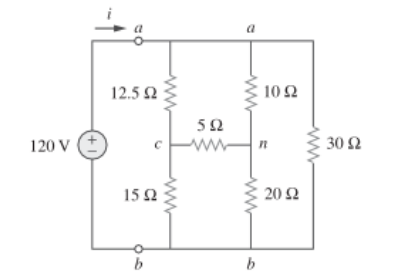
\includegraphics[width=0.48\columnwidth]{circuito1}
    \caption{Circuito original para la conversión estrella-triángulo}
    \label{fig:circuito1}
\end{figure}

\subsubsection{Simulación}
El circuito fue simulado utilizando el software \textit{Qucs-S}, obteniendo los resultados que se 
muestran en la Fig.~\ref{fig:sim1}.

\begin{figure}[H]
    \centering
    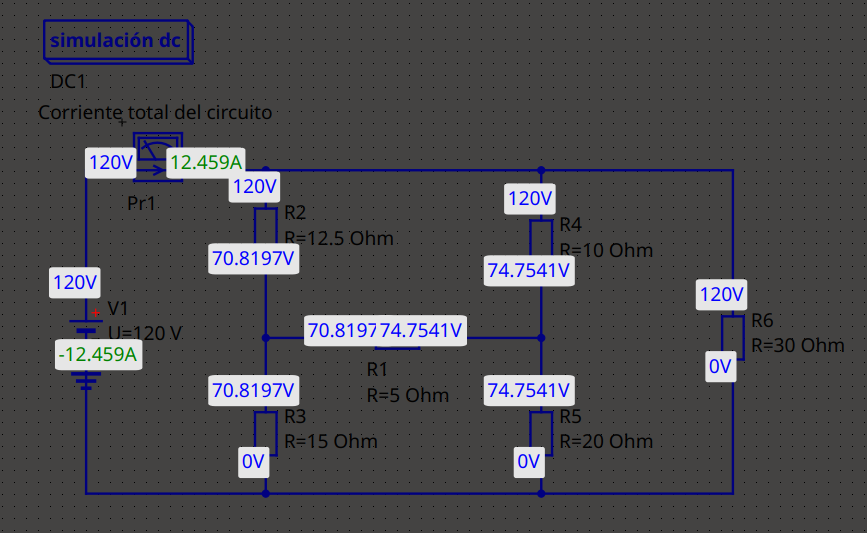
\includegraphics[width=0.48\columnwidth]{simulacion1}
    \caption{Resultados obtenidos en la simulación}
    \label{fig:sim1}
\end{figure}

\subsubsection{Cálculos matemáticos}

\paragraph{Resistencias equivalentes}
Aplicando las fórmulas de conversión estrella-triángulo, se obtienen:

\begin{align*}
R_a &= \frac{R_{ac} \cdot R_{an}}{R_{ac} + R_{an} + R_{cn}} 
     = \frac{12.5 \cdot 10}{12.5 + 10 + 5}
     = \frac{125}{27.5}
     = 4.545\,\Omega \\
R_c &= \frac{R_{ac} \cdot R_{cn}}{R_{ac} + R_{an} + R_{cn}} 
     = \frac{12.5 \cdot 5}{27.5}
     = 2.273\,\Omega \\
R_n &= \frac{R_{an} \cdot R_{cn}}{R_{ac} + R_{an} + R_{cn}} 
     = \frac{10 \cdot 5}{27.5}
     = 1.818\,\Omega
\end{align*}

\paragraph{Simplificación del circuito}
Luego de la conversión, el circuito equivalente se representa en la Fig.~\ref{fig:simplificado1}.

\begin{figure}[H]
\centering
\begin{circuitikz}[american]
    \draw (0,0) to[V=120V] (0,3)
    to[R=4.545$\Omega$] (2.5,3)
    to[R=2.273$\Omega$] (2.5,1.5)
    to[R=15$\Omega$] (2.5,0);

    \draw (2.5,3) -- (4.5,3)
    to[R=1.818$\Omega$] (4.5,1.5)
    to[R=20$\Omega$] (4.5,0);

    \draw (4.5,3) -- (6,3)
    to[R=30$\Omega$] (6,0);

    \draw (0,0) -- (6,0);
\end{circuitikz}
\caption{Circuito equivalente tras la conversión}
\label{fig:simplificado1}
\end{figure}

Las resistencias en serie se combinan:

\begin{align*}
R_1 &= 2.273 + 15 = 17.273\,\Omega \\
R_2 &= 1.818 + 20 = 21.818\,\Omega
\end{align*}

\paragraph{Resistencia equivalente y corriente}

Primero, se calcula la combinación en paralelo:

\begin{align*}
R_{par} &= \frac{R_1 \cdot R_2}{R_1 + R_2} 
        = \frac{17.273 \cdot 21.818}{17.273 + 21.818} 
        \approx 9.64\,\Omega
\end{align*}

Luego, la resistencia total en la rama:

\begin{align*}
R_{\text{rama}} &= 4.545 + 9.64 = 14.185\,\Omega
\end{align*}

\begin{figure}[H]
\centering
\begin{circuitikz}[american]
    \draw (0,0) to[V=9V, invert] (0,3)
    to[R=14.185$\Omega$] (3,3) -- (3,0) -- (0,0);
    \draw (3,3) to[R=30$\Omega$] (3,0);
\end{circuitikz}
\caption{Circuito final equivalente}
\end{figure}

Finalmente, la resistencia equivalente total es:

\begin{align*}
R_{eq} &= \frac{14.185 \cdot 30}{14.185 + 30} 
       \approx 9.63\,\Omega
\end{align*}

Y la corriente total del circuito:

\begin{align*}
I &= \frac{V}{R_{eq}} = \frac{9}{9.63} \approx 12.46\,\text{A}
\end{align*}

%Esto es para ubicarme y separar los ejercicios, no es parte del informe

\subsection{Ejercicio 2: Divisor de voltaje y corriente}

\subsubsection{Ejercicio 2.1: Divisor de voltaje}

\begin{figure}[H]
    \centering
    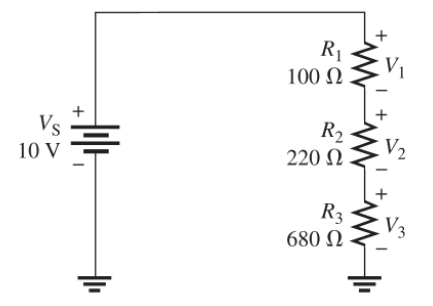
\includegraphics[width=0.48\columnwidth]{circuito2_1}
    \caption{Circuito para divisor de voltaje}
\end{figure}

\paragraph{Montaje físico}
Se realizó el montaje del circuito utilizando resistencias de 100 $\Omega$, 220 $\Omega$ 
y 680 $\Omega$ para las ramas del circuito, y se alimentó con una bateria de 9V. 

\begin{figure}[H]
\centering
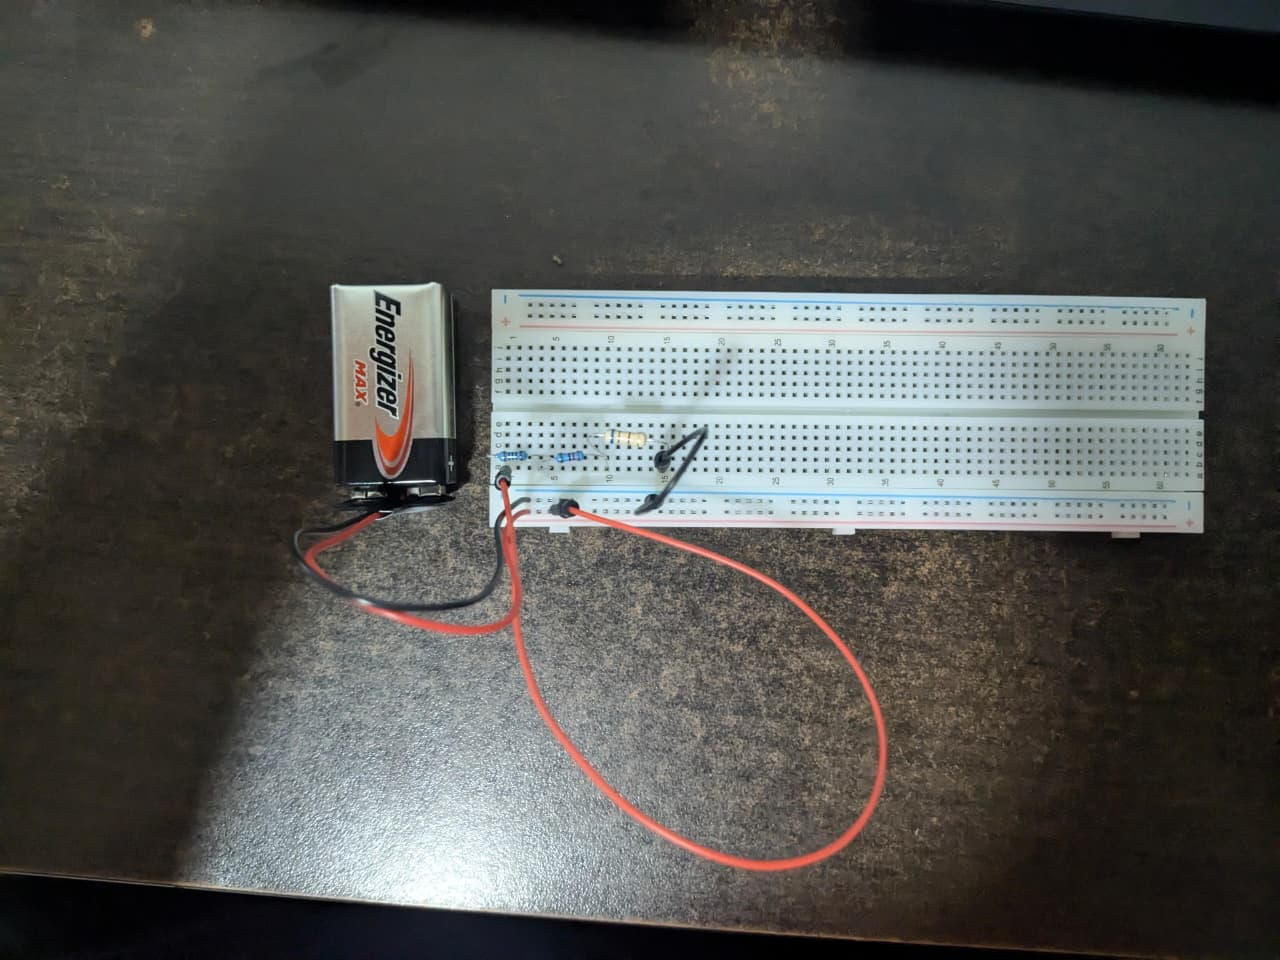
\includegraphics[width=0.5\columnwidth]{montaje2-1}
\caption{Montaje físico del circuito}
\end{figure}

\paragraph{Simulacion del circuito 2.1}
El circuito fue simulado utilizando el software \textit{Qucs}, obteniendo los resultados que se 
muestran en la Fig.~\ref{fig:sim2_1}.
\begin{figure}[H]
    \centering
    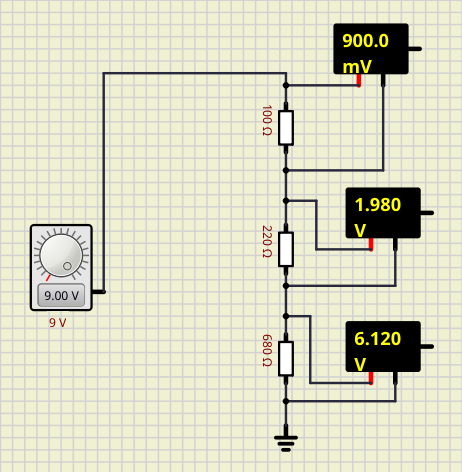
\includegraphics[width=0.48\columnwidth]{simulacion2-1}
    \caption{Resultados obtenidos en la simulación del circuito 2.1}
    \label{fig:sim2_1}
\end{figure}

\paragraph{Cálculos Matemáticos}
Para un circuito en serie, las caídas de tensión pueden determinarse directamente usando el 
principio de divisor de voltaje:

\begin{equation}
V_n = V_S \cdot \frac{R_n}{R_T}
\end{equation}

donde $R_T$ es la resistencia total:

\begin{equation*}
R_T = 100\,\Omega + 220\,\Omega + 680\,\Omega = 1000\,\Omega
\end{equation*}

Aplicando la fórmula para cada resistencia:

\begin{align*}
V_1 &= 9 \cdot \frac{100}{1000} = 9 \cdot 0.1 = 0.9\,\text{V} \\
V_2 &= 9 \cdot \frac{220}{1000} = 9 \cdot 0.22 = 1.98\,\text{V} \\
V_3 &= 9 \cdot \frac{680}{1000} = 9 \cdot 0.68 = 6.12\,\text{V}
\end{align*}

\subsubsection{Verificación}
La suma de las caídas de tensión es:

\begin{equation*}
V_1 + V_2 + V_3 = 0.9 + 1.98 + 6.12 = 9\,\text{V}
\end{equation*}

Lo cual coincide con el voltaje de la fuente, verificando la Ley de Voltajes de Kirchhoff (LVK).

\paragraph{Mediciones}
Se midieron los voltajes en cada rama del circuito utilizando un multímetro, 
obteniendo los siguientes resultados:
\begin{figure}[H]
\centering
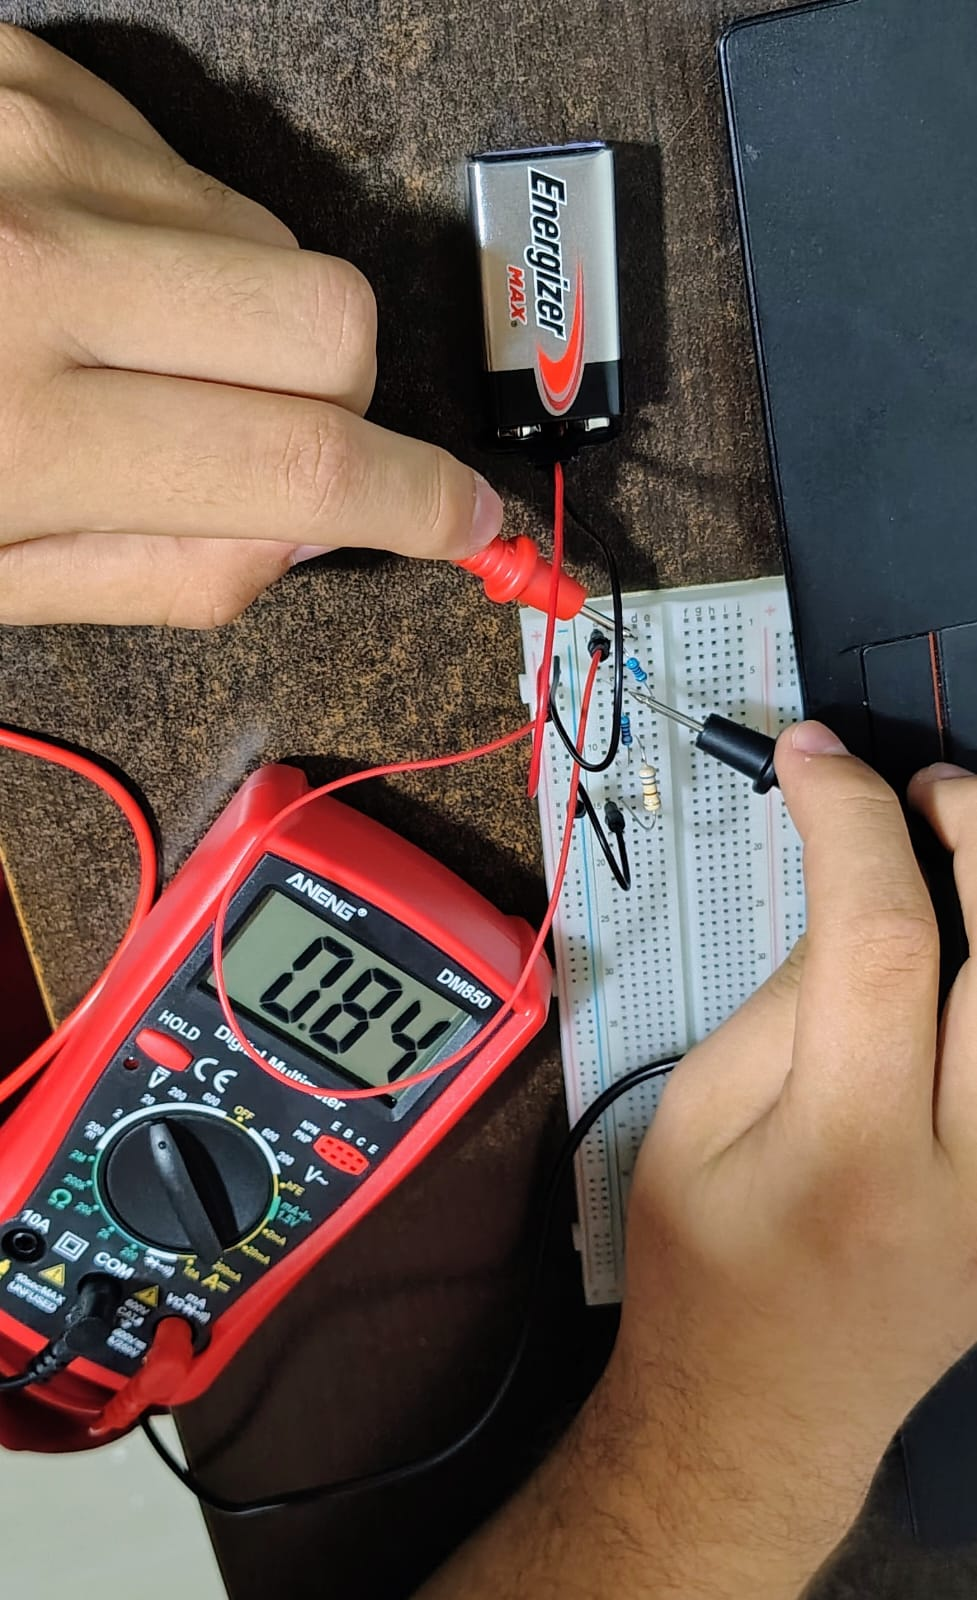
\includegraphics[width=0.3\columnwidth]{medicion2_1_R1}
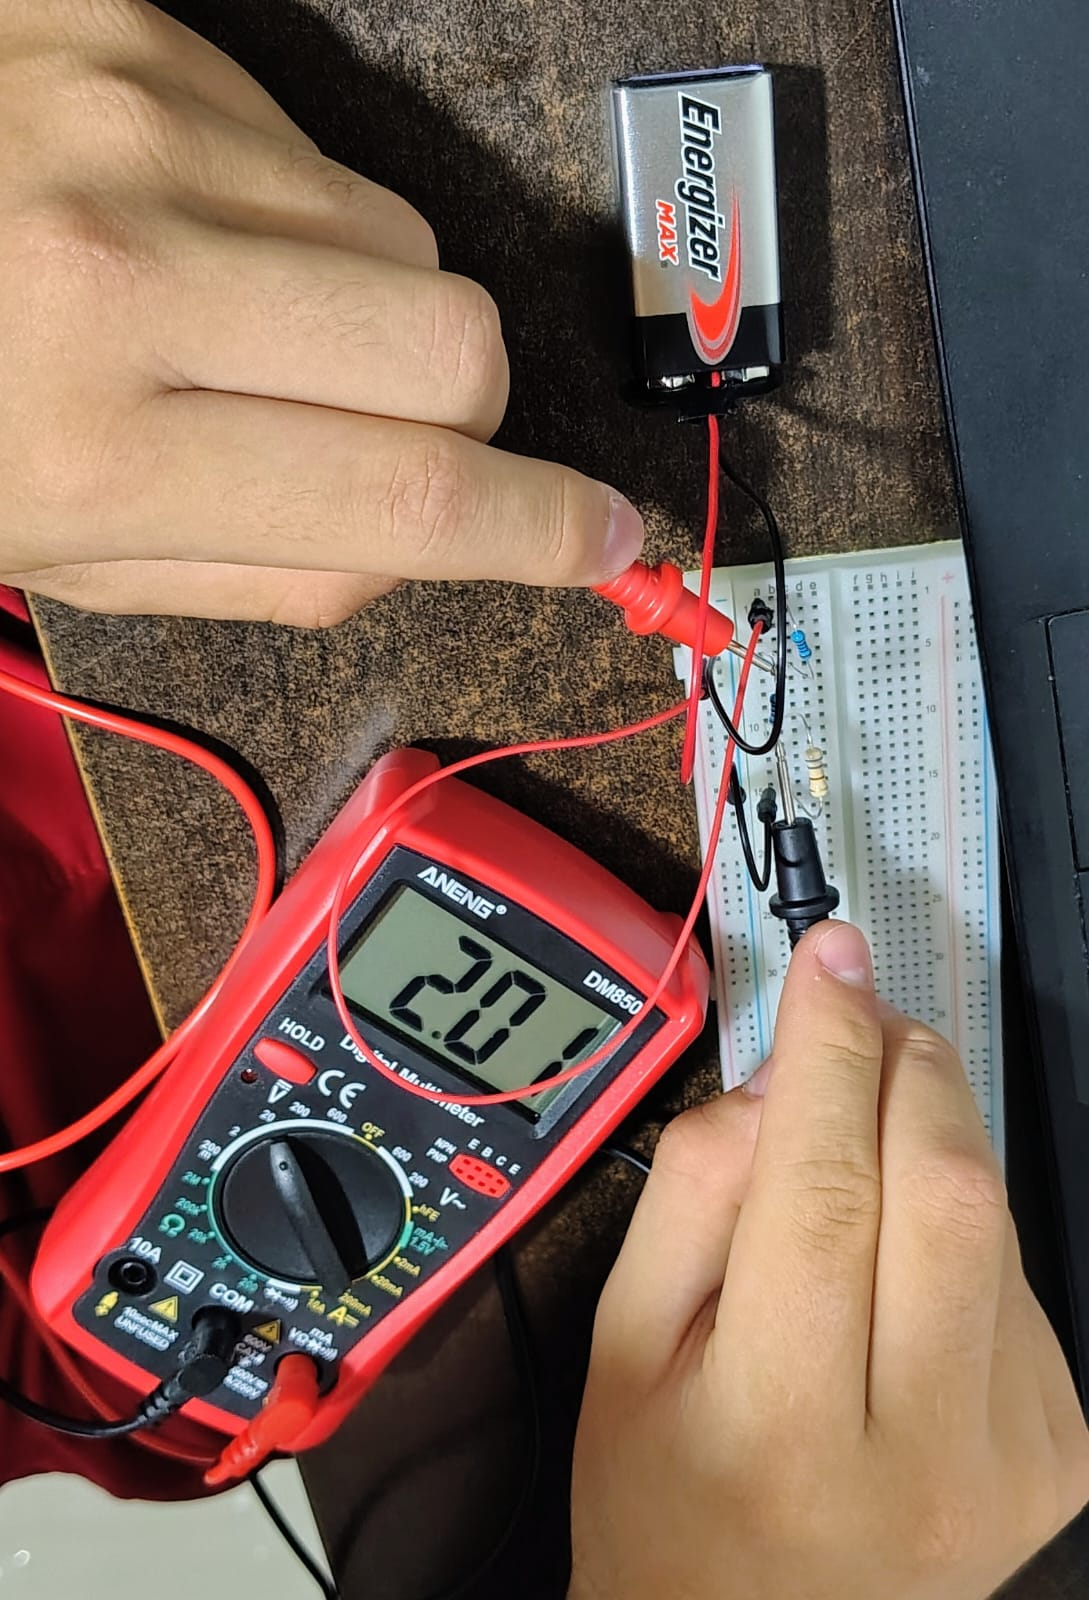
\includegraphics[width=0.3\columnwidth]{medicion2_1_R2}
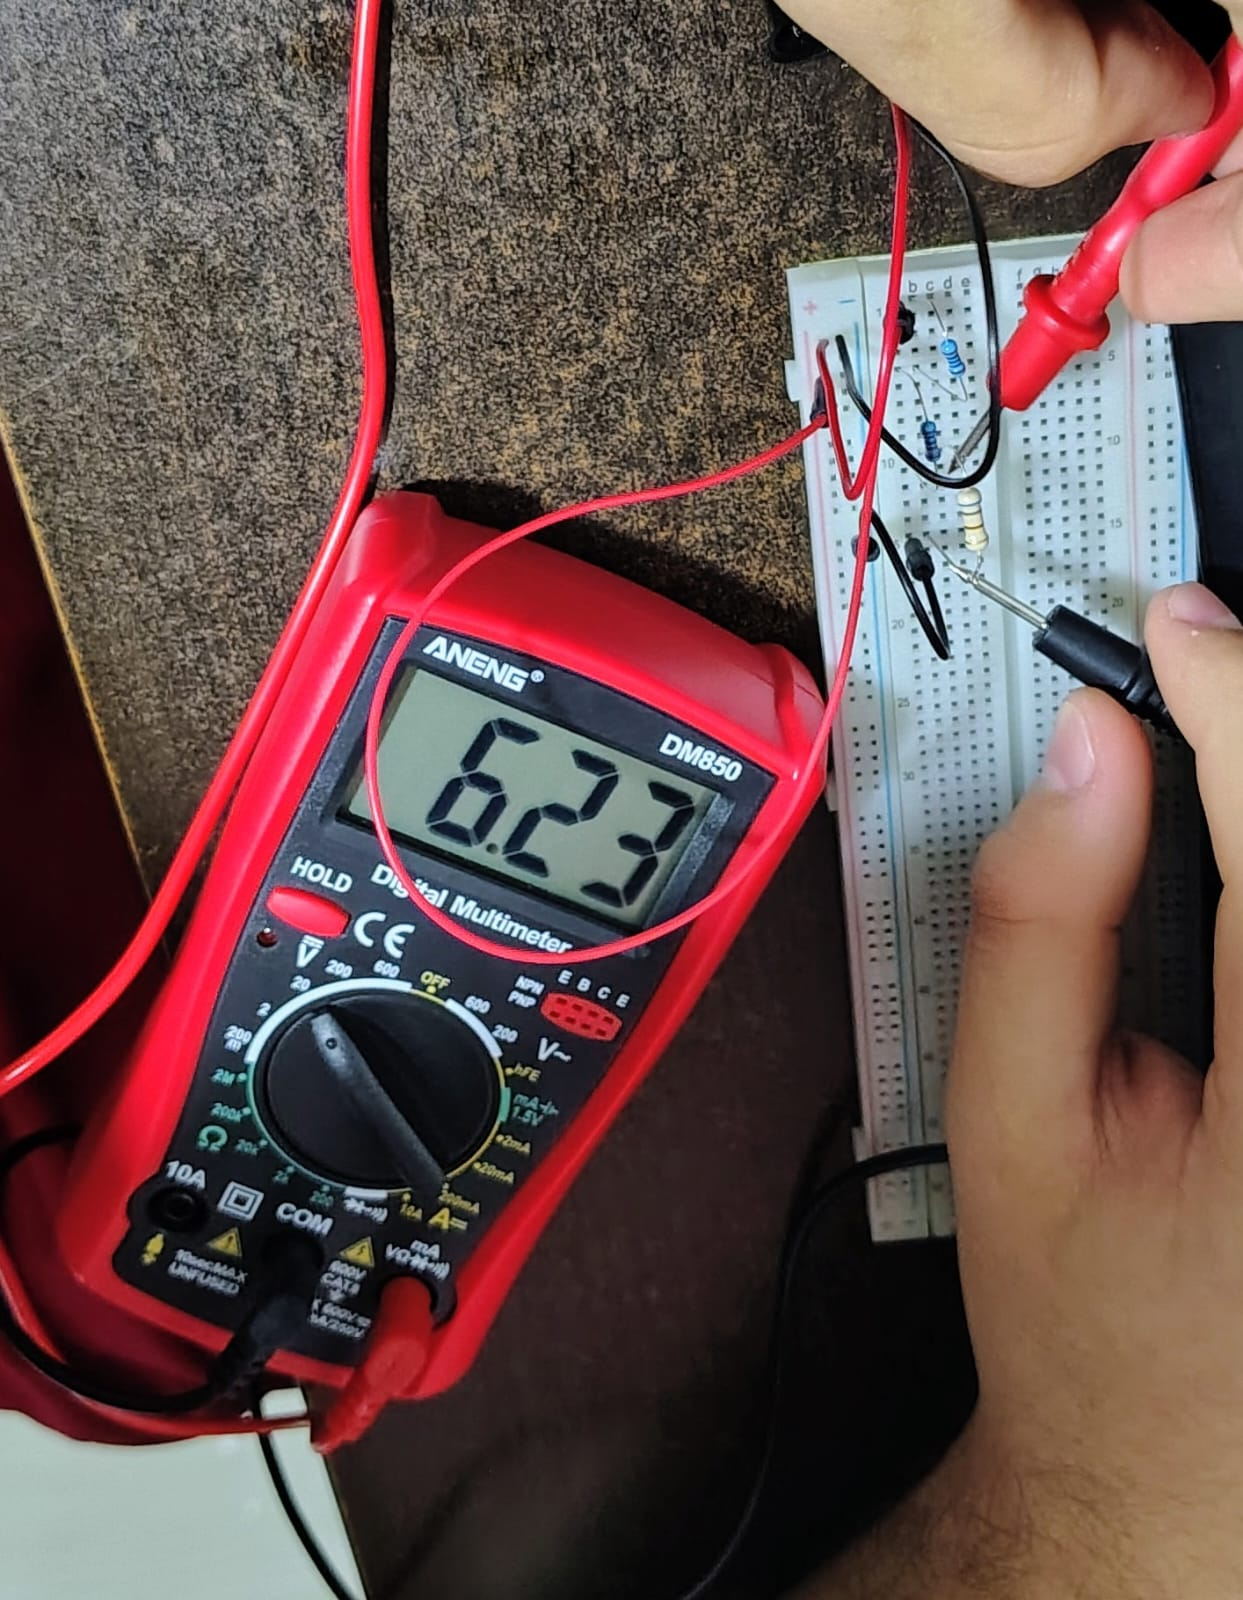
\includegraphics[width=0.3\columnwidth]{medicion2_1_R3}
\caption{Mediciones de voltaje en R1, R2 y R3}
\end{figure}

Los resultados obtenidos fueron:
\begin{itemize}
    \item $V_1 = 0.84\,\text{V}$
    \item $V_2 = 2.01\,\text{V}$
    \item $V_3 = 6.23\,\text{V}$
\end{itemize}
Datos que se aproximan a los resultados teóricos, con pequeñas variaciones debido a 
tolerancias en las resistencias y mediciones.

%Otro ejercicio para ubicarme y separar los ejercicios, no es parte del informe

\subsubsection{Ejercicio 2.2 Divisor de corriente}

\begin{figure}[H]
    \centering
    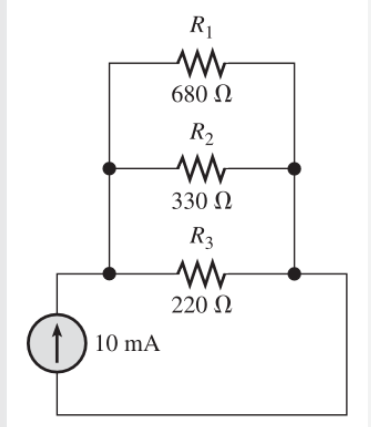
\includegraphics[width=0.48\columnwidth]{circuito2_2}
    \caption{Circuito para divisor de corriente}
\end{figure}

\paragraph{Montaje fisico del circuito 2.2:}
Se realizó el montaje del circuito utilizando resistencias de 220 $\Omega$, 330 $\Omega$
y 680 $\Omega$ para las ramas del circuito, y se alimentó con una bateria de 9V.

\begin{figure}[H]
\centering
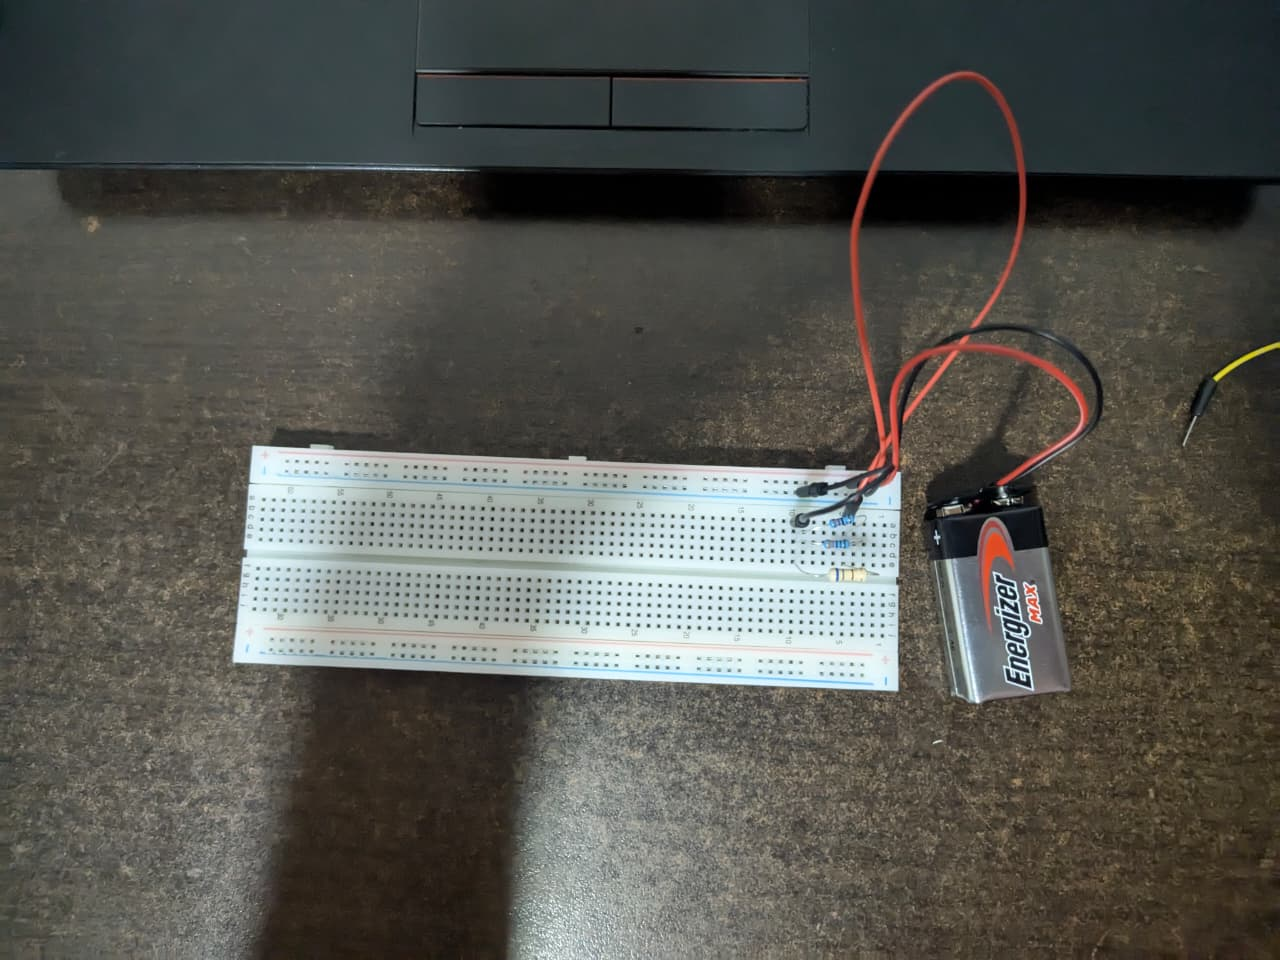
\includegraphics[width=0.5\columnwidth]{montaje2-2}
\caption{Montaje físico del circuito}
\end{figure}

\paragraph{Simulación del circuito 2.2:}
El circuito fue simulado utilizando el software \textit{Qucs-S}, obteniendo los resultados que se 
muestran en la %Fig.~\ref{fig:sim2_2}.

\begin{figure}[H]
  \centering
  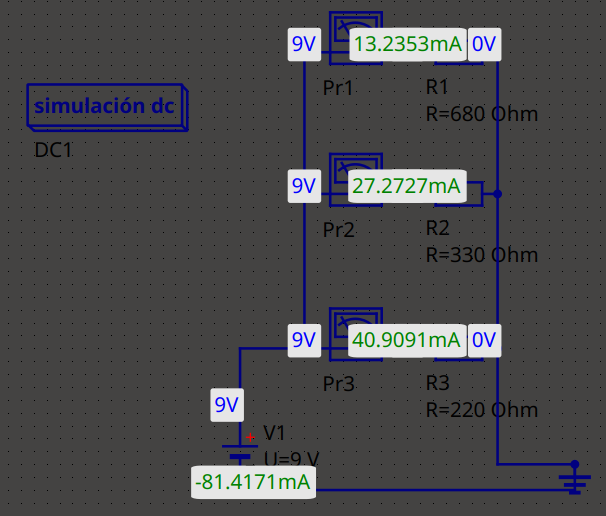
\includegraphics[width=0.48\columnwidth]{simulacion2-2}
  \caption{Resultados obtenidos en la simulación del circuito 2.2}
  \label{fig:sim2_2}
\end{figure}

\paragraph{Cálculos matemáticos}
%Falta el desarrollo de los cálculos matemáticos para el divisor de corriente.

\paragraph{Mediciones}
Se midieron las corrientes en cada rama del circuito utilizando un multímetro,
obteniendo los siguientes resultados:

\begin{figure}[H]
  \centering
  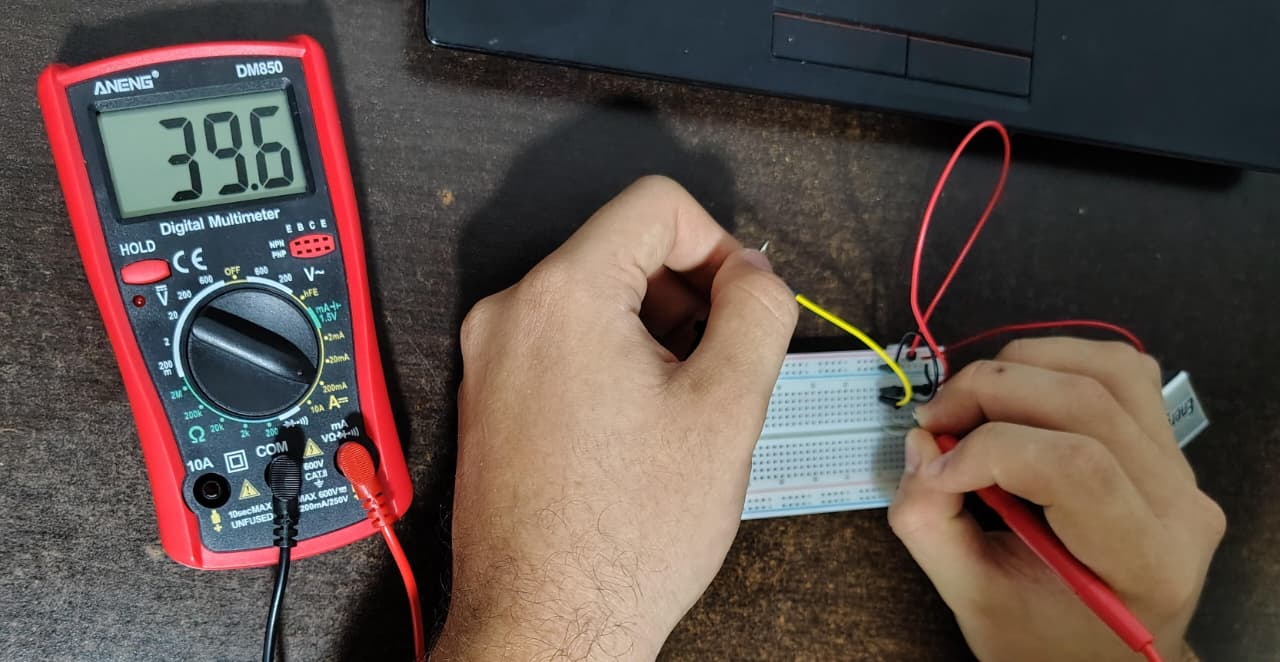
\includegraphics[width=0.3\columnwidth]{medicion2_2_R1}
  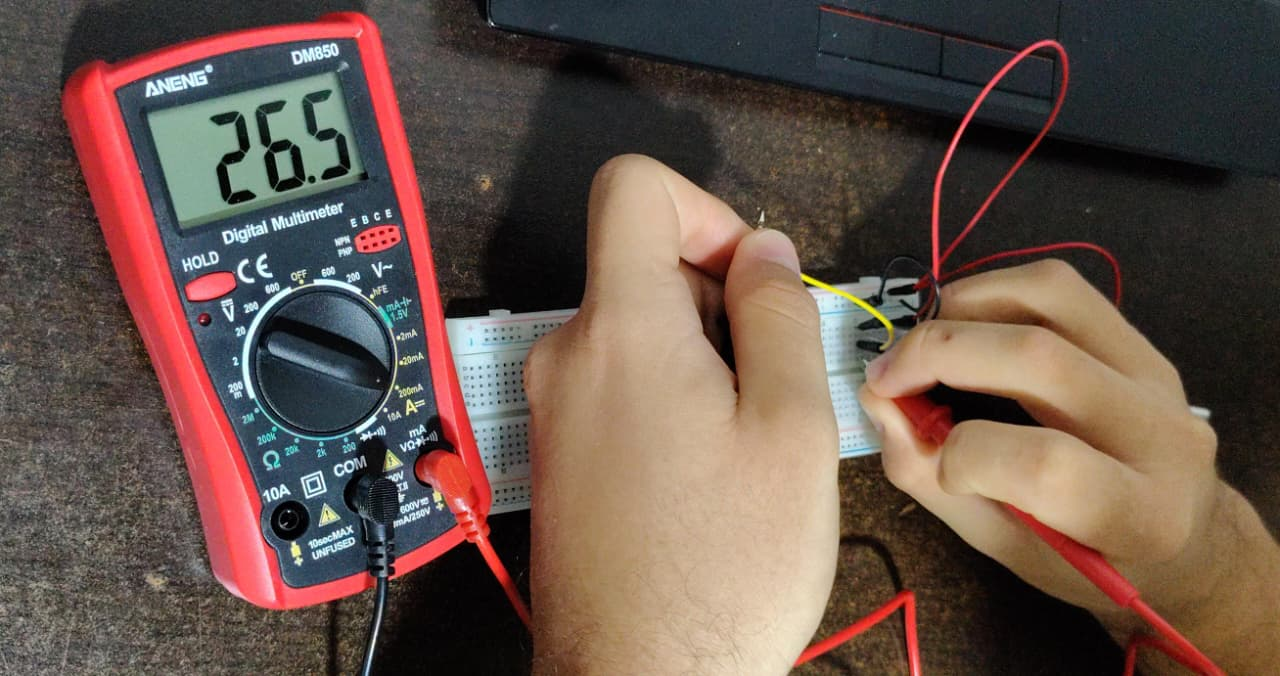
\includegraphics[width=0.3\columnwidth]{medicion2_2_R2}
  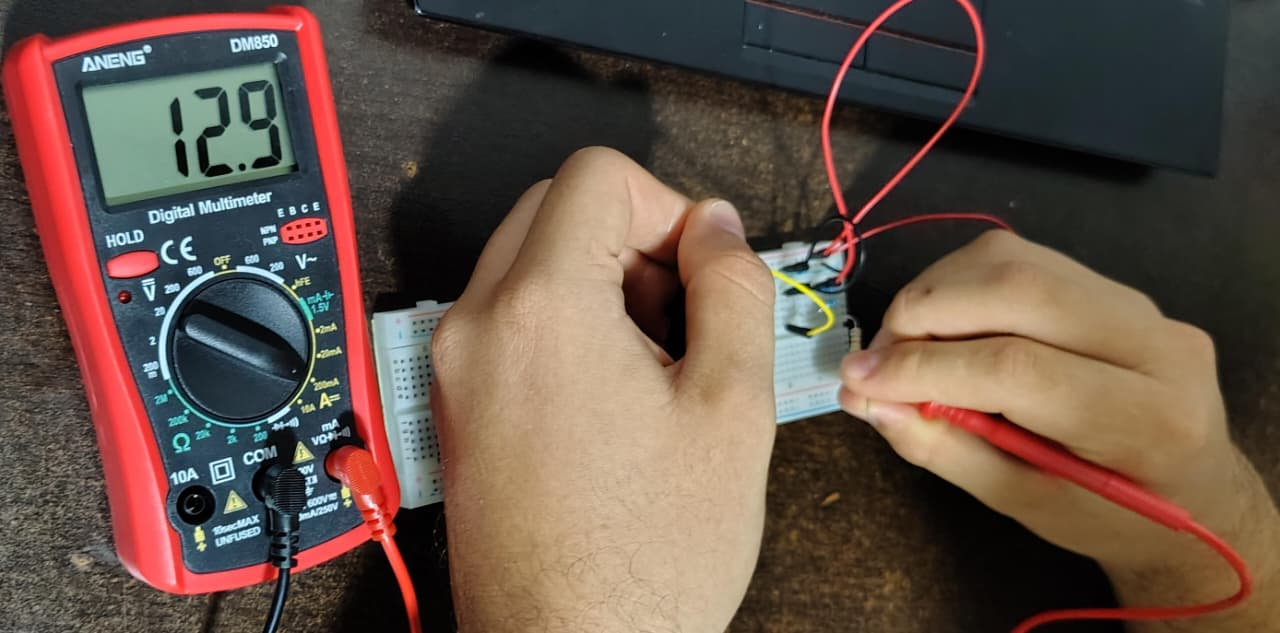
\includegraphics[width=0.3\columnwidth]{medicion2_2_R3}
  \caption{Mediciones de corriente en R1, R2 y R3}
\end{figure}

Los resultados obtenidos fueron:

\begin{itemize}
    \item $I_1 = 39.6\,\text{mA}$
    \item $I_2 = 26.5\,\text{mA}$
    \item $I_3 = 12.9\,\text{mA}$
\end{itemize}

Datos que se aproximan a los resultados teóricos, con pequeñas variaciones debido a
tolerancias en las resistencias y mediciones.

\subsection{Ejercicio 3: Ley de Voltaje de Kirchoff}

\subsubsection{Planteamiento}
Se realizan los cálculos, el montaje y la simulación del circuito,
debido a limitaciones para poder conseguir una resistencia de $180
\Omega$ como indica el ejercicio, cambiamos dicha resistencia por una
de $150 \Omega$

\begin{figure}[H]
  \centering
  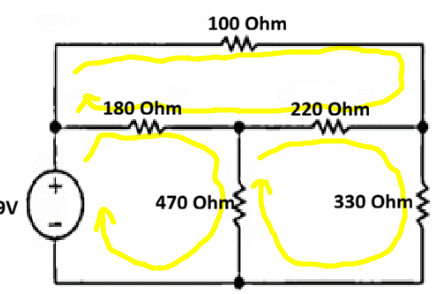
\includegraphics[width=0.48\columnwidth]{circuito3}
  \caption{Circuito para resolver mediante la ley de Kirchoff}
\end{figure}

\subsubsection{Cálculos matemáticos}

\paragraph{Determinantes del sistema 3x3}
Para este circuito se ha designado a la malla que contiene la fuente
de 9V como la Malla1, la malla superior como la Malla 2 y la malla
inferior derecha como la Malla 3. Iniciando los cálculos para la malla 1:

\begin{align*}
  -9 + 150(I_1 - I_2) + 470(I_1 - I_3) = 0 \\
  -9 + 150I_1 - 150I_2 + 470I_1 - 470I_3 = 0 \\
  -9 + 620I_1 - 150I_2 - 470I_3 = 0 \\
  620I_1 - 150I_2 - 470I_3 = 9
\end{align*}

Esa será nuestra ecuación número 1, procediendo con la malla 2:

\begin{align*}
  100I_2 + 220(I_2 - I_3) + 150(I_2 - I_1) = 0 \\
  100I_2 + 220I_2 - 220I_3 + 150I_2 - 150I_1 = 0 \\
  470I_2 - 220I_3 - 150I_1 = 0 \\
  -150I_1 + 470I_2 - 220I_3 = 0
\end{align*}

Esa será la segunda ecuación, procediendo con tercera y última malla:

\begin{align*}
  330I_3 + 470(I_3 - I_1) + 220(I_3 - I_2) = 0 \\
  330I_3 + 470I_3 - 470I_1 + 220I_3 - 220I_2 = 0 \\
  1020I_3 - 470I_1 - 220I_2 = 0 \\
  -470I_1 - 220I_2 + 1020I_3 = 0
\end{align*}

Esa es la tercera ecuación, para encontrar los valores de las
intensidades, se hará uso de una matriz y será resuelta usando el
método de Cramer, la matriz será:

\begin{equation}
  \begin{vmatrix}
    620 && -150 && -470 \\
    -150 && 470 && -220 \\
    -470 && -220 && 1020
  \end{vmatrix}
\end{equation}

Repetimos los valores de las dos primeras ecuaciones para resolver
usando diagonales:

\begin{equation}
  \begin{vmatrix}
    620 && -150 && -470 \\
    -150 && 470 && -220 \\
    -470 && -220 && 1020 \\
    620 && -150 && -470 \\
    -150 && 470 && -220
  \end{vmatrix}
\end{equation}

Así tenemos que el determinante será:

\begin{align*}
  \begin{split}
    \Delta_1 = 620 \cdot 470 \cdot 1020 + [(-150) \cdot \\
    (-220) \cdot (-470)] + [(-470) \cdot (-150) \cdot (-220)]
  \end{split} \\ \\
  \begin{split}
    \Delta_1 = 297,228,000 + (-15,510,000) + (-15,510,000)
  \end{split} \\ \\
  \begin{split}
    \Delta_1 = 266,208,000
  \end{split}
\end{align*}

\begin{align*}
  \begin{split}
    \Delta_2 = (-470) \cdot 470 \cdot (-470) + [(-220) \cdot \\
    (-220) \cdot 620] + [1020 \cdot (-150) \cdot (-150)]
  \end{split} \\ \\
  \begin{split}
    \Delta_2 = 103,823,000 + 30,008,000 + 22,950,000
  \end{split} \\ \\
  \begin{split}
    \Delta_2 = 156,781,000
  \end{split}
\end{align*}

\begin{align*}
  \begin{split}
    \Delta = \Delta_1 - \Delta_2
  \end{split} \\ \\
  \begin{split}
    \Delta = 266,208,000 - 156,781,000
  \end{split} \\ \\
  \begin{split}
    \Delta = 109,427,000
  \end{split}
\end{align*}

Ahora, calculamos el determinante para $I_1$:

\begin{align*}
  \Delta_{I_1} =
  \begin{split}
    \begin{vmatrix}
      9 && -150 && -470 \\
      0 && 470 && -220 \\
      0 && -220 && 1020
    \end{vmatrix}
  \end{split} \\ \\
  \Delta_{I_1} =
  \begin{split}
    \begin{vmatrix}
      9 && -150 && -470 \\
      0 &&  470 && -220 \\
      0 && -220 && 1020 \\
      9 && -150 && -470 \\
      0 &&  470 && -220
    \end{vmatrix}
  \end{split} \\ \\
  \begin{split}
    \Delta_{I_1} = 4,314,600 + 0 + 0 - (0 + 435,600 + 0) \\
    \Delta_{I_1} = 4,314,600 - 435,600 \\
    \Delta_{I_1} = 3,879,000
  \end{split}
\end{align*}

Con la $\Delta_{I_1}$ podemos hallar el valor de $I_1$:

\begin{equation*}
  I_1 = \frac{\Delta_{I_1}}{\Delta} = \frac{3,879,000}{109,427,000} = 0.035448
\end{equation*}

Esto confirma que la corritente en la malla 1 es de $0.035448$ amperios, lo que se 
traduce a $30.448$ mA. Ahora, se calculará la corriente de la malla 2:

Hallamos el determinante de $I_2$:

\begin{align*}
  \Delta_{I_2} =
  \begin{split}
    \begin{vmatrix}
      620  && 9 && -470 \\
      -150 && 0 && -220 \\
      -470 && 0 && 1020
    \end{vmatrix}
  \end{split} \\ \\
  \Delta_{I_2} =
  \begin{split}
    \begin{vmatrix}
      620  && 9 && -470 \\
      -150 && 0 && -220 \\
      -470 && 0 && 1020 \\
      620  && 9 && -470 \\
      -150 && 0 && -220
    \end{vmatrix}
  \end{split} \\ \\
  \begin{split}
    \Delta_{I_2} = 0 + 0 + 930,600 - (0 + 0 - 1,377,000) \\
    \Delta_{I_2} = 930,600 + 1,377,000 \\
    \Delta_{I_2} = 2,307,600
  \end{split}
\end{align*}

Con la $\Delta_{I_2}$ podemos hallar el valor de $I_2$:

\begin{equation*}
  I_2 = \frac{\Delta_{I_2}}{\Delta} = \frac{2,307,600}{109,427,000} = 0.021088
\end{equation*}

La corriente en la malla 2 es de $0.021088$ amperios, que se pueden expresar como 
$21.088$ mA, finalmente calculamos la corriente para la malla 3:

Hallamos el determinante de $I_3$:

\begin{align*}
  \Delta_{I_3} =
  \begin{split}
    \begin{vmatrix}
       620 && -150 && 9 \\
      -150 &&  470 && 0 \\
      -470 && -220 && 0
    \end{vmatrix}
  \end{split} \\ \\
  \Delta_{I_3} =
  \begin{split}
    \begin{vmatrix}
       620 && -150 && 9 \\
      -150 &&  470 && 0 \\
      -470 && -220 && 0 \\
       620 && -150 && 9 \\
      -150 &&  470 && 0
    \end{vmatrix}
  \end{split} \\ \\
  \begin{split}
    \Delta_{I_3} = 0 + 297,000 + 0 - (-1,988,100 + 0 + 0) \\
    \Delta_{I_3} = 297,000 + 1,988,100 \\
    \Delta_{I_3} = 2,285,100
  \end{split}
\end{align*}

Con la $\Delta_{I_3}$ podemos hallar el valor de $I_3$:

\begin{equation*}
  I_3 = \frac{\Delta_{I_3}}{\Delta} = \frac{2,285,100}{109,427,000}  = 0.020882
\end{equation*}

\paragraph{Intensidades del circuito}

Así, concluimos que la corriente en la malla 3 es de $0.020882$ amperios, lo mismo 
que decir $20.882$ mA.

Dado que hay resistencias compartiendo malla, hallamos la intensidad de esas 
resistencias usando los valores encontrados:

\begin{align*}
  I_1 - I_2 = I_{150} \\
  0.035448 - 0.021088 = I_{150} \\
  0.01436 = I_{150} \\ \\
  I_2 - I_3 = I_{220} \\
  0.021088 - 0.020882 = I_{220} \\
  0.000206 = I_{220} \\ \\
  I_1 - I_3 = I_{470} \\
  0.035448 - 0.020882 = I_{470} \\
  0.014566 = I_{470}
\end{align*}

Como se observa el valor de la intensidad para $I_{150}$ es $0.01436$ amperios, lo 
que se expresa como $14.36$ mA, por otro lado, la intensidad para $I_{220}$ es de 
$0.000206$ amperios, se puede expresar como $0.206$ mA, que se puede reexpresar 
como $206 \mu$A, finalmente $I_{470}$ tiene una intensidad de $0.014566$ amperios, 
que se traducen en $14.566$ mA.

\paragraph{Voltajes del circuito}

Usando ley de Ohm con la fórmula del voltaje $V = R \cdot I$ para cada
resistencia en las mallas se pudo calcular los siguientes voltajes:

\begin{align*}
  150 \cdot 0.01436 = V_{R_{150}} \\
  2.154 = V_{R_{150}} \\ \\
  100 \cdot 0.021088 = V_{R_{100}} \\
  2.1088 = V_{R_{100}} \\ \\
  220 \cdot 0.000206 = V_{R_{220}} \\
  0.04532 = V_{R_{220}} \\ \\
  470 \cdot 0.014566 = V_{R_{470}} \\
  6.84 = V_{R_{470}} \\ \\
  330 \cdot 0.020882 = V_{R_{330}} \\
  6.89 = V_{R_{330}}
\end{align*}

Realizamos a su vez, el cálculo de las potencias:

\begin{align*}
  2.154 \cdot 0.01436 = P_{R_{150}} \\
  0.03093 Watts = 30.93 mW = P_{R_{150}} \\ \\
  2.1088 \cdot 0.021088 = P_{R_{100}} \\
  0.04447 Watts = 44.47 mW = P_{R_{100}} \\ \\
  0.04532 \cdot 0.000206 = P_{R_{220}} \\
  0.000009336 Watts = 0.009336 mW = 9.336 \mu W = P_{R_{220}} \\ \\
  6.84 \cdot 0.014566 = P_{R_{470}} \\
  0.09963 Watts = 99.63 mW = P_{R_{470}} \\ \\
  6.89 \cdot 0.020882 = P_{R_{330}} \\
  0.143876 Watts = 143.876 mW = P_{R_{330}}
\end{align*}

\section{Decisiones técnicas}
Se registraron las decisiones técnicas tomadas durante el desarrollo del taller.

\end{document}
